\section{Reducing Monitoring Overheads}
\label{sec:filter}

The instruction-grained monitoring techniques we consider forward all
instructions of certain types (e.g., load instructions) to the monitoring core.
However, not all of these forwarded instructions have relevant monitoring to be
done. For example, for array bounds check, all load and store instructions are
forwarded. However, only loads and stores associated with array pointers have
relevant checking to be done. Thus, we could greatly reduce the amount of
monitoring done by only forwarding instructions that correspond to data that
correspond to array pointers and have been marked with base and bound metadata.
More generally, we can reduce monitoring overheads by filtering out certain
events that correspond to empty (i.e., uninitialized) metadata.

% Overview of inserting dataflow engine
\begin{figure}
  \begin{center}
    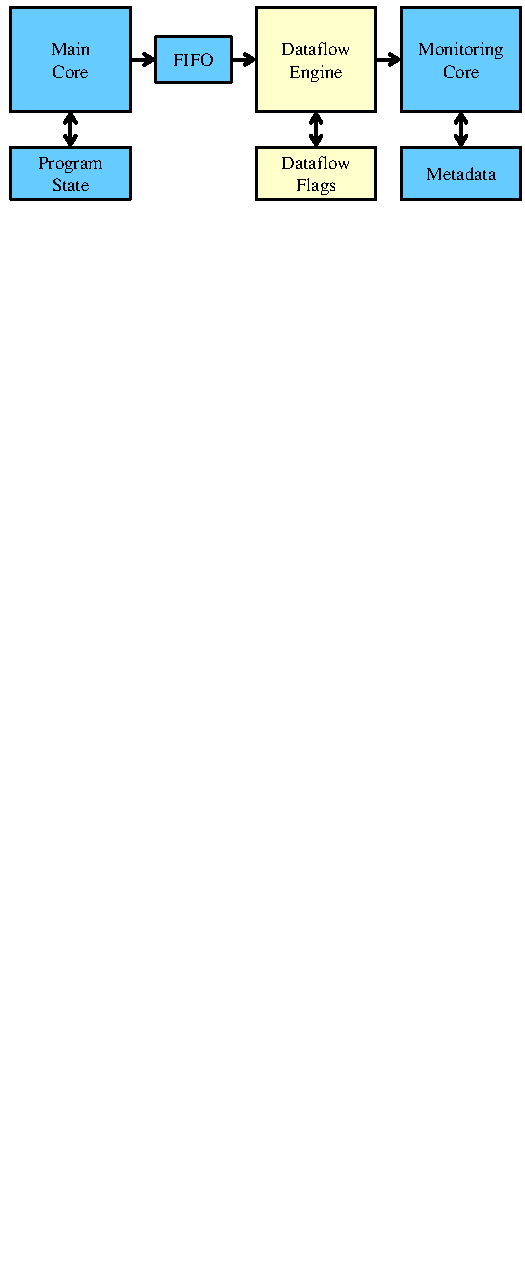
\includegraphics[width=\columnwidth]{figs/dataflow_overview.pdf}
    \vspace{-0.2in}
    \caption{The dataflow engine is inserted between the main core and the monitoring core.}
    \label{fig:filter.overview} 
    \vspace{-0.1in}
  \end{center}
\end{figure}

In this section, we describe how a DIFT-like hardware engine can be used to track
whether metadata has been initialized. We use this information to filter out
monitoring operations for uninitialized metadata. This engine sits between the
main core and the monitoring core (see Figure~\ref{fig:filter.overview}).

\subsection{Initialized Metadata}

% Detailed architecture of dataflow engine
\begin{figure*}
  \begin{center}
    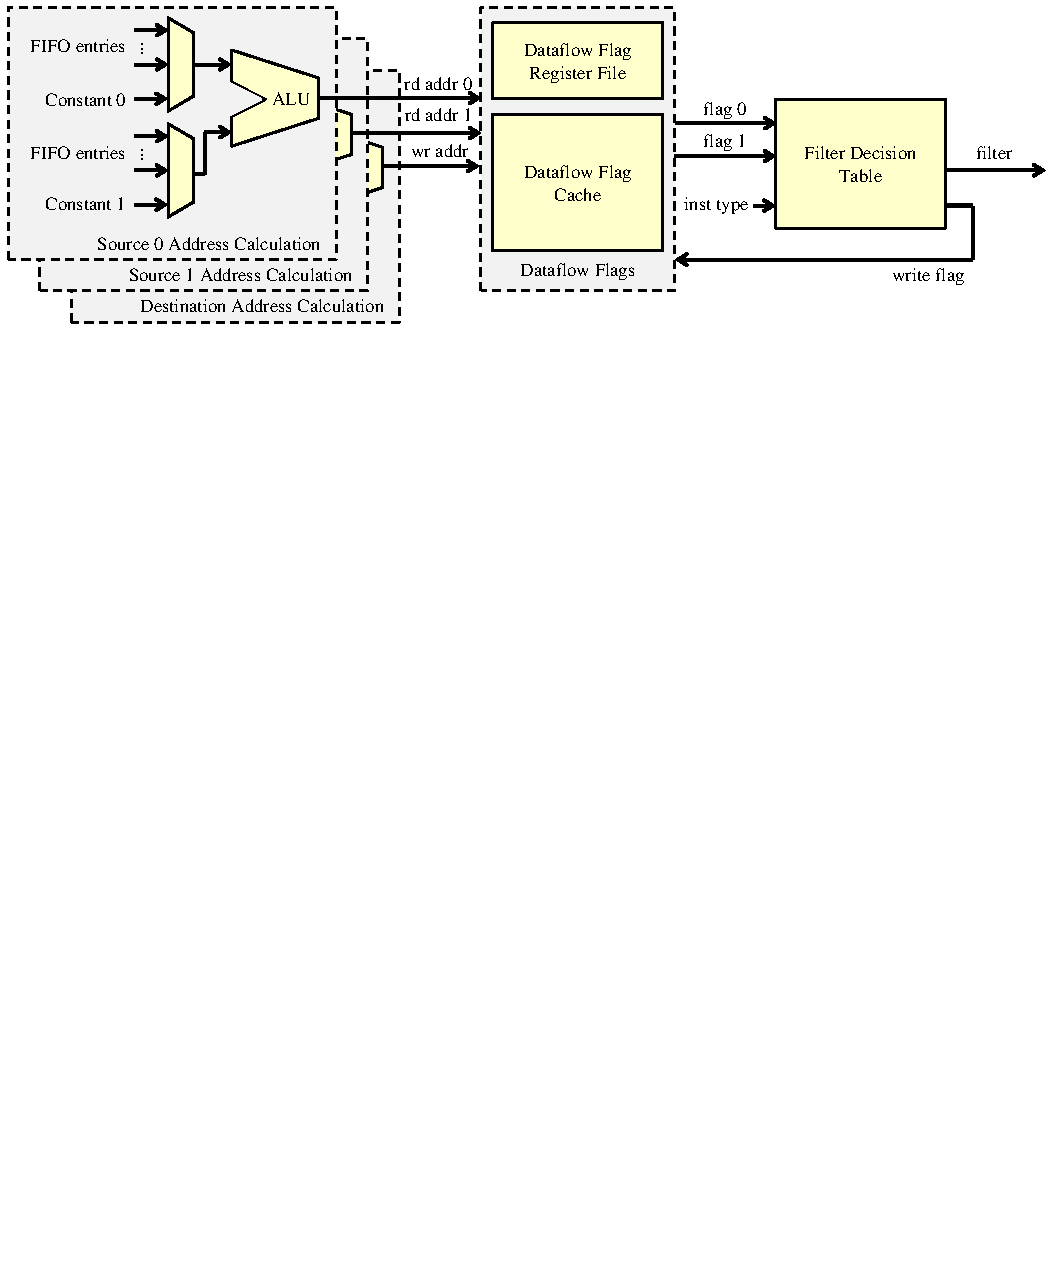
\includegraphics[width=\linewidth]{figs/dataflow_architecture.pdf}
    \vspace{-0.3in}
    \caption{Hardware architecture of dataflow engine.}
    \label{fig:filter.architecture} 
    \vspace{-0.1in}
  \end{center}
\end{figure*}

Figure~\ref{fig:filter.architecture} shows a block diagram of the hardware for keeping track of
initialized metadata. When metadata is initialized, the monitor sends a signal
to the DIFT engine to mark a corresponding initialization flag. Similarly, when
the monitor propagates metadata, it also sends a signal to initialize the
metadata that has been written to. When a new event arrives at the DIFT engine,
it will read in up to two initialization flags. A table is used to configure
which initialization flags should be read in depending on the instruction type of
the event and information from the monitoring event. A pair of simple ALUs is
used to allow calculating memory addresses based on information from the
monitoring event. Typically, the initialization flags read correspond to the
source operands of the monitored instruction.

Given this set of initialization flags, a Filter Decision Table decides, based
on instruction type, whether an event can be filtered out. This table is
configured based on the specific semantics of a monitoring technique.
Typically, if all initialization flags are marked as uninitialized, then the
event can be filtered out. For example, for array bounds check, if the source
register's metadata is marked as uninitialized, then this means that the
register does not correspond to an array pointer. Thus, we can filter out
performing monitoring for this event.

\subsection{Propagating Initialization Flags}

If the source operands are marked as uninitialized, then typically we can
filter out this event. However, in these cases, the monitor also typically
resets the destination operand's metadata as cleared or uninitialized.
Thus, when we filter out one of these events, we need to also propagate the
uninitialized flag to the destination. The Filter Decision Table includes this
information about whether the destination operand metadata should be marked as
uninitialized.
